%% Template para dissertação/tese na classe UFBAthesis
%% versão 1.0
%% (c) 2005 Paulo G. S. Fonseca
%% (c) 2012 Antonio Terceiro
%% (c) 2014 Christina von Flach
%% www.dcc.ufba.br/~flach/ufbathesis

%% Carrega a classe ufbathesis
%% Opções: * Idiomas
%%           pt   - português (padrão)
%%           en   - inglês
%%         * Tipo do Texto
%%           bsc  - para monografias de graduação
%%           msc  - para dissertações de mestrado (padrão)
%%           qual - exame de qualificação de mestrado
%%           prop - exame de qualificação de doutorado
%%           phd  - para teses de doutorado
%%         * Um­dia
%%           scr  - para verão eletrônica (PDF) / consulte o guia do usuário
%%         * Estilo
%%           classic - estilo original a la TAOCP (deprecated)
%%           std     - novo estilo a la CUP (padrão)
%%         * Paginação
%%           oneside - para impressão em face única
%%           twoside - para impressão em frente e verso (padrão)
\documentclass[bsc, classic, a4paper, oneside]{ufbathesis}

%% Preambulo:
\usepackage{xcolor}
\hypersetup{
  colorlinks,
  linkcolor={red!30!black},
  citecolor={blue!50!black},
  urlcolor={blue!80!black}
}
\usepackage[utf8]{inputenc}
\usepackage{graphicx,url}
\usepackage{caption}
\usepackage{lipsum}
\usepackage{amsmath}
\usepackage{mathtools}
\usepackage{enumitem}
\graphicspath{{assets/}}
\usepackage{algorithm2e}
\usepackage{qtree}
\SetKwRepeat{Do}{do}{while} % Macro to allow do while in algorithm2e
\SetAlgorithmName{Algoritmo}{Lista de Algoritmos}

% ---
% Citacao direta com mais de 3 linhas - ABNT NBR 10520/2002 - 5.3
\newlength{\ABNTEXcitacaorecuo}% recuo de 4 cm da margem esquerda
\setlength{\ABNTEXcitacaorecuo}{4cm}
\newcommand{\ABNTEXfontereduzida}{\footnotesize}
\newenvironment*{citacao}[1][default]
{
  \list{}%
  \ABNTEXfontereduzida%
  \addtolength{\leftskip}{\ABNTEXcitacaorecuo}%
  \item[]%
  %\begin{SingleSpace}%
  %\ifthenelse{\not\equal{#1}{default}}{\itshape\selectlanguage{#1}}{}%
}
{ 
  %\end{SingleSpace}%
  \endlist%
}


% Universidade
\university{UNIVERSIDADE FEDERAL DA BAHIA}

% Endereço (cidade)
\address{Salvador}

% Instituto ou Centro Acadêmico
\institute{INSTITUTO DE MATEMÁTICA}

% Nome da biblioteca - usado na ficha catalográfica
\library{BIBLIOTECA REITOR MAC\^{E}DO COSTA}

% Programa de pós-graduação
\program{Programa de Graduação em Ciência da Computação}

% Area de titulação
\majorfield{CI\^{E}NCIA DA COMPUTA\c{C}\~{A}O}

% Titulo da dissertação
\title{Uma abordagem híbrida fuzzy para organização flexível de documentos}

% Data da defesa
% e.g. \date{19 de fevereiro de 2003}
\date{1 de junho de 2016}

% Autor
% e.g. \author{Jose da Silva}
\author{Nilton Vasques Carvalho Junior}

% Orientador(a)
% Opção: [f] - para orientador do sexo feminino
% e.g. \adviser[f]{Profa. Dra. Maria Santos}
\adviser[f]{Profa. Dra. Tatiane Nogueira Rios}

% Orientador(a)
% Opção: [f] - para orientador do sexo feminino
% e.g. \coadviser{Prof. Dr. Pedro Pedreira}
% Comente se não se aplicar
%\coadviser{NOME DO(DA) CO-ORIENTADOR(A)}

%% Inicio do documento
\begin{document}

\pgcompfrontpage{}

%% Parte pre-textual
\frontmatter

\pgcomppresentationpage

% Ficha catalográfica
\authorcitationname{Carvalho, Nilton Vasques Jr.} % e.g. Terceiro, Antonio Soares de Azevedo
\advisercitationname{Rios, Tatiane Nogueira} % e.g. Chavez, Christina von Flach Garcia
\catalogtype{Monografia (Graduação)} % e.g. ``Tese (Doutorado)''
\catalogtopics{``1. Fuzzy C Means. 2. Organização flexível de documents. 3. Lógica Fuzzy. 4. Mineração de dados.''} % e.g. ``1. Complexidade Estrutural. 2. Engenharia de Software''
\catalogcdd{NUMERO CDD} % e.g. ``CDD 20.ed. XXX.YY'' (esse número vai lhe ser dado pela biblioteca)
\catalogingsheet

% Termo de aprovação
\approvalsheet{Salvador, DIA de MES de ANO}{
   \comittemember{Profa. Dra. Tatiane Nogueira Rios}{Universidade Federal da Bahia}
   \comittemember{Prof. Dr. Professor 2}{Universidade 123}
   \comittemember{Profa. Dra. Professora 3}{Universidade ABC}
}

% Dedicatória
% Comente para ocultar
\begin{dedicatory}
Coloque sua DEDICATÓRIA AQUI.
\end{dedicatory}

% Agradecimentos
\acknowledgements
Coloque seus AGRADECIMENTOS AQUI.

% Epigrafe
%  \begin{epigraph}[Tarde, 1919]{Olavo Bilac}
%  Ultima flor do Lácio, inculta e bela,\\
%  Es, a um tempo, esplendor e sepultura;\\
%  Ouro nativo, que, na ganga impura,\\
%  A bruta mina entre os cascalhos vela.
%  \end{epigraph}
\begin{epigraph}[1687]{Isaac Newton}
  O que sabemos é uma gota, o que ignoramos é um oceano.
\end{epigraph}

% Resumo em Português
\resumo
%A new powerful and flexible organization of documents can be obtained by mixing fuzzy and possibilistic clustering, in which documents can belong to more than one cluster simultaneously with different compatibility degrees with a particular topic. The topics are represented by clusters and the clusters are identified by one or more descriptors extracted by a proposed method. We aim to investigate whether the descriptors extracted after fuzzy and possibilistic clustering improves the flexible organization of documents. Experiments were carried using a collection of documents and we evaluated the descriptors ability to capture the essential information of the used collection. The results prove that the fuzzy possibilistic clusters descriptors extraction is effective and can improve the flexible organization of documents.

Diante da grande quantidade de informações geradas e armazenadas pela humanidade na atualidade, 
vários métodos foram propostos visando processar esses dados. Dentre esses dados, temos uma imensa
quantidade de dados textuais, que por sua vez são não estruturados. Com isso é notória a importância,
de organizar de maneira automatizada, esses documentos pelos assuntos ao qual se tratam. Em particular temos um conjunto de técnicas pertencentes ao campo de estudo da mineração de textos, que visam realizar a tarefa de extrair informações relevantes de documentos textuais. Esta tarefa de análise e extração de informações é 
comumente segmentada nas tarefas de coleta, pré-processamento dos documentos, agrupamento dos dados
e por fim a extração de descritores dos grupos obtidos na etapa de agrupamento. Os métodos de agrupamento podem ser separados então pela lógica matemática utilizada, que pode ser a lógica clássica ou a lógica fuzzy. Na lógica clássica, após o agrupamento, cada documento só poderá pertencer a um grupo, enquanto na lógica fuzzy, a pertinência do documento será distribuída entre os grupos. 
Se analisarmos a diversidade de conteúdo em documentos textuais, é trivial notar que frequentemente
um texto aborda um ou mais temas. Com isso é evidente a necessidade de desenvolver-se técnicas para
organizar de maneira flexível os documentos. Percebe-se então, que os métodos de agrupamento fuzzy,
se mostram coerentes com a realidade multi temática dos documentos textuais. Por sua vez, o método FCM(fuzzy c means), que é uma adaptação do clássico k means, se propõe a identificar e separar uma coleção de documentos em grupos, respeitando a lógica multi valorada, permitindo assim que um documento pertença a um ou mais grupos. No entanto o FCM possui algumas falhas conhecidas, o que motivou a pesquisa e desenvolvimento de métodos alternativos e baseados no FCM, com o propósito de sanar estes problemas. Este é o caso dos métodos PCM(Possibilístico C Means) e PFCM(Possibilístico C Means). 
Para então avaliarmos corretamente o resultado do agrupamento e a qualidade da organização flexível 
de documentos, é preciso extrair corretamente os descritores dos grupos obtidos, levando em 
consideração a relevância de determinado termo para cada grupo. Com isso temos um cenário no qual é 
preciso combinar métodos de agrupamento fuzzy com métodos de extração de descritores, para obtermos
uma bom resultado no processo de organização dos documentos. A investigação e refinamento dessa 
combinação de métodos, foi a motivação do presente trabalho. Como resultado desse trabalho foi,
proposto extender os experimentos referentes a organização flexível de documentos, utilizando
novos métodos de agrupamento fuzzy existentes na literatura, como o PCM e o PFCM. Assim como também 
foi proposto os métodos de extração de descritores: i) Mixed-PFDCL 
({ \it Mixed - Possibilistic Fuzzy Descriptor Comes Last\/ }), que se utiliza da abordagem híbrida do 
algoritmo PFCM, misturando assim descritores fuzzy e possibilísticos. ii) MixedW-PFDCL
({ \it Mixed Weighted - Possibilistic Fuzzy Descriptor Comes Last\/ }), 
onde além de misturar descritores 
fuzzy e possibilístico, leva em consideração os parâmetros de ponderação do método PFCM.
Além dos métodos de extração de descritores, foi conduzido um estudo dos impactos de se utilizar o 
algoritmo PCM, no método de agrupamento hierárquico HFCM, o que resultou no método de 
agrupamento hierárquico HPCM ({ \it Hierarchical Possibilistic C Means\/ }).
% FALAR SOBRE OS MÈTODOS FUZZY UTILIZADOS, FCM, PFCM, PCM, HFCM, HPCM
% FALAR SOBRE A EXTRAÇÂO DE DESCRITORES
% FALAR SOBRE A MISTURA REALIZADA NA EXTRAÇÃO DE DESCRITORES

% Palavras-chave do resumo em Português
\begin{keywords}
agrupamento fuzzy, agrupamento possibilístico, organização flexível de documentos, 
mineração de textos
\end{keywords}

% Resumo em Ingles
\abstract
A new powerful and flexible organization of documents can be obtained by mixing fuzzy and possibilistic clustering, in which documents can belong to more than one cluster simultaneously with different compatibility degrees with a particular topic. The topics are represented by clusters and the clusters are identified by one or more descriptors extracted by a proposed method. We aim to investigate whether the descriptors extracted after fuzzy and possibilistic clustering improves the flexible organization of documents. Experiments were carried using a collection of documents and we evaluated the descriptors ability to capture the essential information of the used collection. The results prove that the fuzzy possibilistic clusters descriptors extraction is effective and can improve the flexible organization of documents.

% Palavras-chave do resumo em Ingles
\begin{keywords}
fuzzy clustering, possibilistic clustering, flexible organization, documents, text mining
\end{keywords}

% Sumario / Índice
% Comente para ocultar
\tableofcontents

% Lista de figuras
% Comente para ocultar
\listoffigures

% Lista de tabelas
% Comente para ocultar
\listoftables

%% Parte textual
\mainmatter

% Eh aconselhável criar cada capitulo em um arquivo separado, digamos
% "capitulo1.tex", "capitulo2.tex", ... "capituloN.tex" e depois
% inclui-los com:
% \include{capitulo1}
% \include{capitulo2}
% ...
% \include{capituloN}
%
% Importante: Use \xchapter ao invés de \chapter, se quiser colocar texto antes do inicio do capitulo.

\xchapter{Introdução}{Uma breve introdução sobre do que se trata esta monografia e a maneira como o texto está organizado.}

%A new powerful and flexible organization of documents can be obtained by mixing fuzzy and possibilistic clustering, in which documents can belong to more than one cluster simultaneously with different compatibility degrees with a particular topic. The topics are represented by clusters and the clusters are identified by one or more descriptors extracted by a proposed method. We aim to investigate whether the descriptors extracted after fuzzy and possibilistic clustering improves the flexible organization of documents. Experiments were carried using a collection of documents and we evaluated the descriptors ability to capture the essential information of the used collection. The results prove that the fuzzy possibilistic clusters descriptors extraction is effective and can improve the flexible organization of documents.

Diante da grande quantidade de informações geradas e armazenadas pela humanidade na atualidade, 
vários métodos foram propostos visando processar esses dados. Dentre esses dados, temos uma imensa
quantidade de dados textuais, que por sua vez são não estruturados. Com isso é notória a importância,
de organizar de maneira automatizada, esses documentos pelos assuntos ao qual se tratam. Em particular temos um conjunto de técnicas pertencentes ao campo de estudo da mineração de textos, que visam realizar a tarefa de extrair informações relevantes de documentos textuais. Esta tarefa de análise e extração de informações é 
comumente segmentada nas tarefas de coleta, pré-processamento dos documentos, agrupamento dos dados
e por fim a extração de descritores dos grupos obtidos na etapa de agrupamento. Os métodos de agrupamento podem ser separados então pela lógica matemática utilizada, que pode ser a lógica clássica ou a lógica fuzzy. Na lógica clássica, após o agrupamento, cada documento só poderá pertencer a um grupo, enquanto na lógica fuzzy, a pertinência do documento será distribuída entre os grupos. 
Se analisarmos a diversidade de conteúdo em documentos textuais, é trivial notar que frequentemente
um texto aborda um ou mais temas. Com isso é evidente a necessidade de desenvolver-se técnicas para
organizar de maneira flexível os documentos. Percebe-se então, que os métodos de agrupamento fuzzy,
se mostram coerentes com a realidade multi temática dos documentos textuais. Por sua vez, o método FCM(fuzzy c means), que é uma adaptação do clássico k means, se propõe a identificar e separar uma coleção de documentos em grupos, respeitando a lógica multi valorada, permitindo assim que um documento pertença a um ou mais grupos. No entanto o FCM possui algumas falhas conhecidas, o que motivou a pesquisa e desenvolvimento de métodos alternativos e baseados no FCM, com o propósito de sanar estes problemas. Este é o caso dos métodos PCM(Possibilístico C Means) e PFCM(Possibilístico C Means). 
Para então avaliarmos corretamente o resultado do agrupamento e a qualidade da organização flexível 
de documentos, é preciso extrair corretamente os descritores dos grupos obtidos, levando em 
consideração a relevância de determinado termo para cada grupo. Com isso temos um cenário no qual é 
preciso combinar métodos de agrupamento fuzzy com métodos de extração de descritores, para obtermos
uma bom resultado no processo de organização dos documentos. A investigação e refinamento dessa 
combinação de métodos, foi a motivação do presente trabalho. Como resultado desse trabalho foi,
proposto extender os experimentos referentes a organização flexível de documentos, utilizando
novos métodos de agrupamento fuzzy existentes na literatura, como o PCM e o PFCM. Assim como também 
foi proposto os métodos de extração de descritores: i) Mixed-PFDCL 
({ \it Mixed - Possibilistic Fuzzy Descriptor Comes Last\/ }), que se utiliza da abordagem híbrida do 
algoritmo PFCM, misturando assim descritores fuzzy e possibilísticos. ii) MixedW-PFDCL
({ \it Mixed Weight - Possibilistic Fuzzy Descriptor Comes Last\/ }), 
onde além de misturar descritores 
fuzzy e possibilístico, leva em consideração os parâmetros de ponderação do método PFCM.
Além dos métodos de extração de descritores, foi conduzido um estudo dos impactos de se utilizar o 
algoritmo PCM, no método de agrupamento hierárquico HFCM, o que resultou no método de 
agrupamento hierárquico HPCM ({ \it Hierarchical Possibilistic C Means\/ }).
% FALAR SOBRE OS MÈTODOS FUZZY UTILIZADOS, FCM, PFCM, PCM, HFCM, HPCM
% FALAR SOBRE A EXTRAÇÂO DE DESCRITORES
% FALAR SOBRE A MISTURA REALIZADA NA EXTRAÇÃO DE DESCRITORES


\xchapter{Fundamentação Teórica}{Este capítulo tem como objetivo fundamentar as bases necessárias dos campos de estudos utilizados nesta monografia.}

\section{Lógica Fuzzy}
\section{Pré-Processamento}
\section{Agrupamento Fuzzy}
\section{Extração de descritores}


\xchapter{Trabalhos Relacionados}{Trabalhos relacionados a organização flexível de documentos e
sistemas de recuperação de informação.}

% Strings de busca 
%
% (((((clustering) OR cluster labeling) OR cluster description) AND fuzzy AND( document OR text
% mining)))
% http://ieeexplore.ieee.org/search/searchresult.jsp?queryText=(((((clustering)%20OR%20cluster%20labeling)%20OR%20cluster%20description)%20AND%20fuzzy%20%20AND(%20document%20OR%20text%20mining)))&ranges=2010_2016_Year&matchBoolean=true&searchField=Search_All

% ((clustering OR "cluster label*" OR "cluster descriptors") AND fuzzy AND (document OR "text
% mining" OR "document organization" OR "soft document" OR "text data"))
% http://ieeexplore.ieee.org/search/searchresult.jsp?queryText=((clustering%20OR%20.QT.cluster%20label*.QT.%20OR%20.QT.cluster%20descriptors.QT.)%20AND%20fuzzy%20AND%20(document%20OR%20.QT.text%20mining.QT.%20OR%20.QT.document%20organization.QT.%20OR%20.QT.soft%20document.QT.%20OR%20.QT.text%20data.QT.))&sortType=desc_p_Publication_Year&matchBoolean=true&searchField=Search_All

\section{Considerações Iniciais}

A proposta de organização flexível de documentos está relacionada a vários campos de estudo, como
ficou evidenciado na fundamentação teórica. Por isso a literatura existente para essa proposta é
bastante rica e densa. Portanto com o propósito de otimizar a atividade de pesquisa e seleção do
conhecimento científico produzido a respeito do tema, foram utilizados algumas técnicas de revisão
sistemática de literatura ($SLR\ -\ Sistematic\ Literature\ Review$) utilizadas em \cite{Rios2010}.
Com o objetivo de estabelecer critérios mais precisos na fase inicial da descoberta de conteúdo
científico relacionado ao tema. Foi então adotada uma técnica comum ao método SLR, que consiste na
elaboração de uma uma string de busca, usando operadores lógicos. Estabelecendo assim uma maneira
mais objetiva para a obtenção de resultados relevantes a proposta dessa monografia.  Portanto,
levando em consideração os tópicos chaves e a proposta desse trabalho, foi construída a seguinte
string de busca: 

\begin{multline} (clustering\ OR\ "cluster\ label*"\ OR\ "cluster\ descriptors")\ AND\ fuzzy \\ AND\
  (document\ OR\ "text\ mining"\ OR\ "document\ organization"\ OR\ \\ "soft\ document"\ OR\ "text\
data") \label{eq:busca} \end{multline}

Devido o amplo acervo de publicações científicas presentes no repositório
IEEExplore\footnote{http://ieeexplore.ieee.org/}, assim como também a possibilidade de se utilizar
operadores lógicos e buscas parametrizadas. Foi realizado então uma busca no repositório IEEExplore,
restringindo o período de resultados entre os anos de 2010 e 2016, permitindo então que os
resultados obtidos fossem mais recentes.

Com base nos resultados obtidos, foi realizada a leitura dos títulos e resumos dos artigos, com o
propósito de descartar resultados com baixa relevância para essa pesquisa.  Durante a fase de
leitura parcial dos resultados da busca, foram agrupados os artigos em três categorias: agrupamento
fuzzy, extração de descritores e organização flexível de documentos.  As publicações selecionadas e
direcionadas para a categoria de agrupamento fuzzy, foram as que possuíam propostas de alteração de
métodos de agrupamento existentes ou novos métodos. Enquanto artigos que tinham como conteúdo a
análise dos termos de uma coleção, critério de seleção de termos ou atribuição de termos a grupos de
documentos, foram agrupados na categoria de extração de descritores. Por fim, artigos mais gerais,
propondo métodos ou realizando revisões de métodos, pertinentes ao processo de organização de
documentos textuais, foram categorizados no grupo de organização flexível de documentos.

Para complementar os resultados obtidos foram adicionados artigos de alta relevância para o tema, e
que apesar de serem antigos, ainda são amplamente citados em pesquisas recentes. Muitos desses
artigos como é o caso do método FCM proposto em \cite{Bezdek1984}, são pilares fundamentais para o
tema.

Nas próximas seções contém a revisão das pesquisas selecionadas, onde é elucidado os pontos chaves
de cada pesquisa, a definição das propostas contida nos artigos e por fim a conexão com o objetivo
dessa monografia.

\section{Organização Flexível de Documentos}

Após a proposição da lógica fuzzy que se propunha a lidar com a incerteza e imprecisão em
\cite{Zadeh1965}, foi possível a elaboração de diversos métodos que se utilizassem dos benefícios da
lógica fuzzy e aplicassem a diversos problemas do mundo real. Este é o caso da organização de
documentos, que por não ser uma tarefa precisa, necessita de uma certa flexibilidade no processo.

\cite{Matsumoto10} informa que os mecanismos adotados em sistemas de recuperação de informação
(SRI), tais como buscadores web, estão dispostos em dois grupos. Sendo que o primeiro tem como foco
o usuário realizando a busca, a qual é comumente chamada de busca web personalizada.  Nessa
abordagem os resultados obtidos são ordenados de acordo com a relevância do resultado para o
usuário. Para calcular essa relevância, os buscadores realizam tarefas de coleta de dados dos
usuários e comparação das preferências com demais usuários do sistema.  Enquanto na segunda
abordagem os resultados da busca é categorizado em grupos, permitindo assim que o usuário decida em
qual grupo ele pretende visualizar as informações. Por exemplo, quando um usuário pesquisar pelo
termo java, os resultados poderiam ser agrupados nas seções: máquina virtual, linguagem java,
programas em java, oracle e etc. Seguindo essa linha de categorização de resultados em SRIs,
\cite{MarcaciniR10} propõe uma abordagem de agrupamento incremental e hierárquico para construção
dos tópicos dos documentos, a qual permite a atualização das categorias a medida que novos
documentos são adicionados sem realizar a etapa de agrupamento novamente. É possível a visualização
dessa abordagem de categorização hierárquica, através da ferramenta online
Torch\footnote{http://sites.labic.icmc.usp.br/torch/webcluster/}, dos autores do artigo.

Com o surgimento de várias tecnologias, como mídias sociais, computação ubíqua, internet das coisas 
e principalmente os dispositivos móveis, que ultrapassou os 7 bilhões de
dispositivos\footnote{Segundo o relatório do The Mobile Economy disponível em
\url{http://www.gsmamobileeconomy.com/GSMA_Global_Mobile_Economy_Report_2015.pdf}, a quantidade de
dispositivos móveis (smartphones e tablets) atingiu o total de 7,517 bilhões no ano de 2015.} no ano
de 2015. Onde por sua vez, todas essas tecnologias produzem uma abundante quantidade de dados não
estruturados, dificultando a tarefa de métodos de mineração de dados, e por consequência
também os métodos de organização de documentos já existentes. A esse cenário é usualmente atribuído
o nome de $Big\ Data$. Sendo assim novas pesquisas como \cite{Havens2012} e \cite{Kumar2015} tem 
sido conduzidas, focadas em bases com imensas quantidades de dados. Segundo \cite{Havens2012} 
existem duas abordagens principais para otimizar o agrupamento de dados que se encaixam na categoria
$Very\ Large$ (Tabela \ref{table:datasize}, a primeira consiste na técnica de agrupamento
distribuído incremental e o agrupamento por amostragem progressiva ou aleatória. Nos métodos que
usam a técnica de amostragem, primeiramente é selecionado uma amostra com os dados representativos 
da coleção, depois é realizado o agrupamento, e em seguida é generalizado o agrupamento para o
restante dos dados. Um dos métodos mais populares baseado em amostragem é o algoritmo 
$generalized\ extensible\ fast\ FCM$ (geFFCM)\cite{Havens2012}. O geFFCM utiliza amostragem
progressiva para se obter uma versão reduzida dos dados, de maneira que a mesma preserve as
características da base original. Porém segundo \cite{Havens2012}, a técnica de amostragem do geFFCM
é ineficiente para dados na categoria $Very\ Large$, o que levou os autores a propor uma extensão do
geFFCM com uma melhoria na forma de realizar a amostragem dos dados, utilizando uma metodologia de
seleção aleatória.

\begin{table}[!htp]
  \centering
  \begin{tabular}{ |c|c c c c c|}
    \hline
    Bytes & $10^6$ & $10^8$ & $10^{10}$ & $10^{12}$ & $10^{>12}$ \\
    \hline
    "tamanho" & medium & large & huge & monster & very large \\
    \hline
  \end{tabular}
  \label{table:datasize}
  \caption{Classificação das bases de dados de acordo com o seu tamanho\cite{Havens2012}}
\end{table}

De acordo com \cite{Deng2010}, a organização flexível de dados através do algoritmo FCM possui
uma falta de estabilidade, pois como a inicialização do FCM depende da aleatoriedade, o resultado
final do agrupamento pode variar a cada inicialização. Assim como os dados presentes em bases de
dados textuais são de alta dimensionalidade.  Os autores propuseram então um modelo de inicialização
da partição que extrai da coleção medidas de peso, raio e objetos mais representativos para orientar
a inicialização da partição inicial. A respeito do problema da dimensionalidade, \cite{Deng2010}
sugere a redução da matrix documentos x termos, usando uma medida estatística para avaliar a
qualidade dos termos presentes na coleção, descartando assim os termos considerados de baixa
qualidade e consequentemente reduzindo a largura da matriz.

\cite{Karami2015} propõe um modelo para análise textual de documentos médicos. Um dos pontos
interessantes propostos pelo autor é a utilização do agrupamento fuzzy na etapa de
pré-processamento e ponderação dos termos, antes de realizar o agrupamento e classificação. 
O agrupamento fuzzy é aplicado a coleção de termos presentes na coleção, e ao contrário do
agrupamento na etapa pós processamento, a pertinência ocorre da palavra a um tópico ou grupo, 
de maneira que termos com alta pertinência possuem significados
semânticos mais próximos. Essa aproximação semântica é realizada com base em um vocabulário
predefinido.
 


\xchapter{Abordagem proposta}{Investigação e refinamento do método de organização flexível de documentos}

\section{Considerações inicias}
A organização de uma coleção de documentos em vários tópicos, de modo que exista sobreposição
entre os grupos é um importante problema em sistemas de recuperação de informação(SRIs). Na
literatura diversas estratégias são utilizadas visando otimizar a organização flexível de
documentos, conforme foi abordado no capítulo anterior. Soma-se a isso o fato de que a maioria dos
métodos que adicionam flexibilidade ao processo, como por exemplo  os métodos de agrupamento, nem
sempre são desenvolvidos com o foco em documentos textuais. Que conforme foi abordado ao longo do
texto, possui características que acrescentam algumas dificuldades no processo, tais como a alta
dimensionalidade dos dados, assim como também usualmente são armazenados de maneira não estruturada.
E ainda com o crescente aumento do uso de tecnologias de produção de conteúdo, a quantidade de dados
textuais alcança grandes volumes de dados o que os enquadra no contexto do $Big Data$. 
Portanto esse cenário fortalece a importância de se conduzir pesquisas e investigações em torno da
organização flexível de documentos. Entretanto não é esperado que um método de agrupamento seja
totalmente adequado para todos os tipos de dados, incluindo os dados de alta dimensionalidade como
os dados textuais\cite{Steinbach2004}. Desta maneira esse capítulo tem como objetivo detalhar as 
contribuições
desta monografia a organização flexível de documentos, através da investigação dos impactos de se
utilizar a estratégia de se misturar o agrupamento fuzzy e possibilístico provida pelo algoritmo
PFCM. Onde este método de agrupamento pretende resolver os problemas dos elementos equidistantes e 
dos grupos
coincidentes, apresentados nas partições fuzzy e possibilística respectivamente. 

Conforme observa-se no capítulo 2, o algoritmo PFCM produz duas
partições, sendo um fuzzy e outra possibilística, o que induziu o presente trabalho a propor duas extensões do
método de extração de descritores Soft-wFDCL proposto por \cite{Nogueira2013}, que leva em
consideração apenas os valores de pertinências presentes na partição fuzzy. A primeira extensão
denominada Mixed-PDCL({\it Mixed - Possibilistic Fuzzy Descriptor Comes Last\/}), 
a qual contempla durante a extração de descritores as duas partições do PFCM.
E a segunda proposta é o método 
MixedW-PDCL({\it Mixed Weighted - Possibilistic Fuzzy Descriptor Comes Last\/}), 
que é uma extensão do Mixed-PDCL, porém ponderando as
contribuições das partições com base nos parâmetros $a$ e $b$ do PFCM. A última contribuição é a
proposta do método HPCM, que é uma extensão do método de agrupamento hierárquico HFCM, o qual
utiliza o algoritmo PCM no lugar do FCM para produzir a hierarquia.

Na primeira sessão deste capítulo é apresentado informações das bases de dados utilizadas, com as
suas características, origem e composição dos documentos. Nos capítulos seguintes é definido as
propostas sugeridas por essa monografia. E por fim os dados obtidos com os experimentos realizados.

\section{Informações das bases de dados}

Na mineração de dados e consequentemente nos trabalhos relacionados a organização flexível de
documentos, é comum se realizar a avaliação dos métodos propostos, conduzindo-se experimentos sobre
bases de dados existentes na literatura com essa finalidade\cite{Rossi2013}. Para isso, as bases
precisam estar apresentadas de maneira estruturada. Assim sendo, nesta pesquisa foi adotado o formato
{\it tf-idf\/}(\ref{eq:tfidf}) como forma de estruturar os dados presentes nas bases, 
de modo a capturar a
importância relativa dos termos nos documentos e na coleção. Cada coleção foi então disposta em dois
arquivos, sendo que o arquivo com extensão $.data$ contém $n$ linhas, onde cada linha constitui a 
representação de um
documento da coleção no formato {\it tf-idf\/}, para $n$ igual a quantidade de documentos 
presentes na
coleção, enquanto o que arquivo de extensão $.names$ possui a descrição dos $m$ termos existentes na
coleção dispostos um por linha.

A base Opinosis\footnotemark é composta de opiniões de consumidores a respeito das características de alguns
produtos, obtidas dos portais amazon.com, tripadvisor e edmunds.com. As opiniões presentes na base,
abordam tópicos como serviços de hospedagem, dispositivos eletrônicos e carros. Sendo que no total
as sentenças presentes na coleção estão distribuídas em 51 categorias, onde cada categoria possui
100 sentenças na média. Os dados dessa base
foram obtidos no repositório {\it UCI Machine Learning Repository\/}\cite{Frank2010}, 
que mantém várias coleções de
dados que são utilizados pela comunidade de aprendizado de máquina para a realização de análises
empíricas dos algoritmos.
\footnotetext{\url{http://archive.ics.uci.edu/ml/datasets/Opinosis+Opinion+26frasl3B+Review}}

A coleção de documentos 20Newsgroup\footnotemark original contém aproximadamente 20000 documentos de notícias,
particionados em mais ou menos 20 temas. No entanto para os experimentos realizados nesta pesquisa, 
foi utilizado uma versão mais
compacta da coleção, contendo 2000 documentos pertencentes ao tema ciência, a qual contém os tópicos
sci.space, sci.electronics e sci.med. Esta base tem-se mostrado bastante popular em
aplicações textuais de aprendizado de máquina\cite{Nogueira2015}, tais como agrupamento e 
classificação de textos.
Essa base foi coletada originalmente por Ken Lang para a pesquisa Newsweeder apresentada em
\cite{Lang1995}. 
\footnotetext{\url{http://qwone.com/~jason/20Newsgroups/}}

Os documentos presentes na base de dados Reuters-21578\footnotemark apareceram inicialmente na Reuters newswire
em 1987. Sendo que os documentos foram coletados e indexados diretamente por membros da Reuters e da
{\it Carnegie Group, Inc.} também em 1987 para o desenvolvimento do CONSTRUE\cite{Hayes1990}, que
foi um sistema de categorização de documentos. Onde no ano de 1990 essa base de dados foi tornada
pública pela Reuters, para ser utilizada em pesquisas de recuperação de informação. No entanto as
versões inicias dessa base continham documentos repetidos e ambíguos, o que motivou um grupo de
pesquisadores de categorização textual durante a conferência {\it ACM SIGIR '96\/}, a realizar uma
limpeza na base, possibilitando uma melhor comparação dos resultados entre diferentes estudos. Essa
versão final ficou com o total de 21578 documentos, distribuídos entre 43 diferentes categorias. 
Contudo
nesta pesquisa foi utilizada uma amostragem menor da coleção, contendo 1052 documentos, selecionados
aleatoriamente de cada classe da coleção.
\footnotetext{\url{https://archive.ics.uci.edu/ml/datasets/Reuters-21578+Text+Categorization+Collection}}

A base de dados WAP({\it WebACE Project\/}) é composta de um conjunto de páginas web coletadas por 
\citeonline{Moore1997}, para um projeto de pesquisa de agrupamento, seleção e recuperação de páginas web.
Os dados presentes nesta coleção foram obtidos pelos autores do artigo em 98 páginas web, onde
posteriormente foram distribuídos em 20 diferentes categorias, que abrangem tópicos como negócios e 
finanças, tecnologias, trabalho e
indústria. O conteúdo obtido está disposto em 1560 documentos na sua versão original, sendo que
todos os documentos foram utilizados nessa pesquisa.

A coleção de documentos NSF\footnotemark({\it National Science Foundation\/}) foi obtida do 
repositório de dados para pesquisas de aprendizado de máquina 
{\it UCI Machine Learning Repository}\cite{Frank2010}. O conteúdo dos dados presentes na base é
composto de 129000 resumos, sendo um resumo por documento, descrevendo prêmios da NSF para 
pesquisas básicas. Para os experimentos descritos nesta monografia, foram selecionados 1600 
documentos de maneira aleatória entre as categorias apresentadas na coleção.
\footnotetext{\url{https://archive.ics.uci.edu/ml/datasets/NSF+Research+Award+Abstracts+1990-2003}}

A base de dados Hitech adquirida em \citeonline{Karypis2006}, é parte de uma coleção de bases da 
conferência TREC({\it Text REtrieval Conference\/})\footnotemark. 
\footnotetext{\url{http://trec.nist.gov/data.html}}
Esta base é composta de um conjunto de notícias da revista {\it Jose Mercury News\/}\footnotemark, 
as quais são distribuídos em categorias distintas. As notícias presentes na coleção
abordam temas como computadores, eletrônicos, saúde, medicina, pesquisa e tecnologia. 
A base originalmente possui 2301
documentos, onde para esta pesquisa foram selecionados uma amostragem aleatória contendo 600
documentos. 
\footnotetext{\url{http://www.mercurynews.com/}}

\begin{table}[!htp]
  \centering
  \begin{tabular}{ |c|p{11cm}|}
    \hline
    {\bf documentos} & número de documentos presentes na coleção \\
    \hline
    {\bf termos} & número de termos existentes na coleção após o pré-processamento \\
    \hline
    {\bf \% zeros} & número relativo de zeros na {\it tf-idf\/}, ou seja quantifica o quanto a
matriz é esparsa \\
    \hline
    {\bf classes} & número de classes presentes na coleção \\
    \hline
    {\bf dp-class} & desvio padrão ao se considerar o percentual de documentos que
pertence a determinada classe na coleção \\
    \hline
    {\bf $>$classe} & percentual de documentos pertencentes a maior classe na coleção \\
    \hline
    {\bf n-gramas} & quantidade de termos considerados sequencialmente na coleção \\
    \hline
  \end{tabular}
  \caption{Descrição das características objetivas presentes em coleções textuais elencadas para
este trabalho}
  \label{table:datainfo}
\end{table}

Outro aspecto não menos importante, são as características particulares das coleções de dados. Pois
ressalta-se que para uma mais apurada análise dos resultados, é pertinente considerar as
particularidades de cada base, com a finalidade de encontrar possíveis justificativas para os
resultados apresentados, realizando-se indagações comparativas as peculiaridades sabidamente
conhecidas dos métodos analisados. Portanto o conjunto de características particulares de cada base
obtidos em \citeonline{Rossi2013} e adaptados a esta pesquisa, dar-se à como apresentado
na Tabela (\ref{table:datainfo}). 


Portanto, uma análise objetiva das características presentes nas seis bases descritas anteriormente 
está apresentado na (\ref{table:datasets}). Onde é possível notar de maneira bem 
objetiva ao se observar
a coluna \% zeros da tabela, que todas as bases apresentam uma quantidade de zeros em mais de $90\%$
dos dados, o que caracteriza o peculiar problema dos dados esparsos já caracterizado ao longo do
texto, como algo inerente aos dados textuais.


\begin{table}[!htp]
  \centering
  \begin{tabular}{ |l|c c c c c c c|}
    \hline
    {\bf nome} & docs & termos & classes & \% zeros & dp-classe & $>$classe & n-gramas \\
    \hline
    {\bf Opinosis} & 51 & 842 & 3 & 95,73\% & 0,1 & 96,07\% & 1-grama \\
    \hline
    {\bf 20newsgroups} & 2000 & 11028 & 4 & 99,11\% & 0,1 & 25\% & 1-grama \\
    \hline
    {\bf Hitech} & 600 & 6925 & 6 & 97,93\% & 0,1 & 16,67\% & 1-grama \\
    \hline
    {\bf NSF} & 1600 & 2806 & 16 & 99,76\% & 0,1 & 3,12\% & 1-grama \\
    \hline
    {\bf WAP} & 1560 & 8070 & 20 & 98,51\% & 0,1 & 100\% & 1-grama \\
    \hline
    {\bf Reuters-21578} & 1052 & 3925 & 43 & 98,55\% & 0,1 & 8,55\% & 1-grama \\
    \hline
  \end{tabular}
  \caption{Características das bases de dados utilizadas nesta pesquisa}
  \label{table:datasets}
\end{table}

\section{Refinamento com o algoritmo PFCM}

Conforme ficou evidenciado, a tarefa de organizar de maneira flexível um conjunto de documentos
textuais, possui diversos desafios. Em particular, ao se agrupar um conjunto de documentos é
esperado que os grupos resultantes possuam significado relevante, ou seja o algoritmo de
agrupamento precisa detectar a estrutura natural dos dados\cite{Steinbach2004}. Alguns desses 
desafios está na dificuldade em escalar os métodos usuais para bases de dados na categoria {\it Very Large}
conforme a escala apresentada na Tabela \ref{table:datasize}, assim como também a obtenção de
mecanismos efetivos para se avaliar a qualidade dos grupos produzidos, técnicas para se medir a
interpretabilidade dos resultados, capacidade para estimar os parâmetros dos algoritmos,
possibilidade para funcionar de maneira incremental, reduzindo o custo computacional durante a
atualização dos grupos com novos dados, e também a capacidade de continuar a produzir bons
resultados em cenários compostos de documentos ruidosos \cite{Carvalho2016}. 

Portanto para \citeonline{Steinbach2004}:
\begin{citacao}
  {\it [...] there is no reason to expect that one type of clustering approach will
  be suitable for all types of data, even all high dimensional data. Statisticians and other
  data analysts are very cognizant of the need to apply different tools for different types of
  data, and clustering is no different\/}.
\end{citacao}

Diante então dos desafios propostos, e com a evidência de que é possível aprimorar os resultados, ao
se utilizar novas estratégias de agrupamento. A investigação apresentada nesta seção tem como
objetivo analisar de qual forma a organização de documentos pode ser otimizada, ao aplicar na etapa
de agrupamento uma estratégia que misture as partições possibilística e fuzzy, através do algoritmo
PFCM. A escolha desse algoritmo foi feita devido o seu potencial para absorver as qualidades
presentes no FCM contrabalanceando as suas deficiências ao agregar também o PCM e sua partição
possibilística. Outro ponto a se considerar são as diversas pesquisas na literatura abordando o
desempenho do PFCM, 
como por exemplo em \citeonline{Pal2005,Yan2009,Kumar2010,Grover2014,Popescu2015}.

Com isso foi conduzido um experimento adaptando a estratégia de organização flexível de documentos
definida em \citeonline{Nogueira2013},
utilizando na etapa de agrupamento o método PFCM. Porém esse método produz duas partições uma
possibilística e uma partição fuzzy. Desse modo foi aplicado o método de extração de descritores
Soft-wFDCL na partição fuzzy e outra vez na partição possibilística, produzindo assim dois grupos de
descritores. Essa adaptação está ilustrada na Figura (\ref{fig:flexibleorganization}).

\begin{figure}[!htp] 
  \centering
  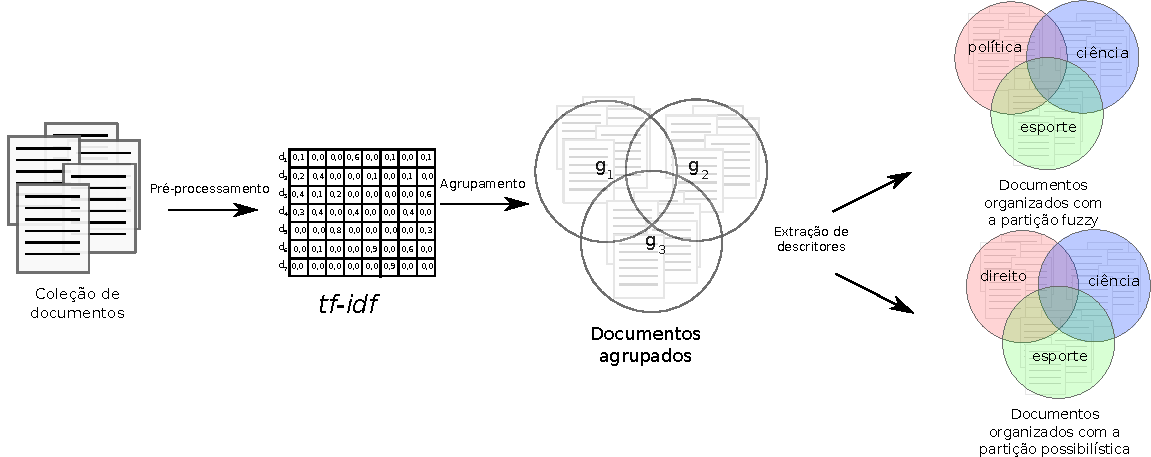
\includegraphics[width=1.0\columnwidth]{assets/process_pfcm.pdf} 
  \caption{Estratégia de organização flexível de documentos adotada ao se misturar abordagens fuzzy
  e possibilísticas no agrupamento} 
  \label{fig:flexibleorganization} 
\end{figure}

Para se calcular a quantidade ótima de grupos, para cada base de dados foi utilizado o
método da silhueta fuzzy (equação \ref{eq:fs}), método bastante utilizado com o propósito de avaliar
o agrupamento de documentos. Assim sendo, o número ideal de grupos é determinado após a execução da
silhueta fuzzy variando o número de grupos entre 2 e o número de classes de cada coleção.
Ressalta-se que em coleções que os dados não possuem rótulos, ou seja o número de classes é
desconhecido, ainda é possível usar o método da silhueta fuzzy para definir o número ótimo de
grupos. No entanto, a quantidade máxima de grupos deve ser definida de modo empírico ou com base em
alguma informação prévia a respeito dos dados. 

Para permitir uma análise comparativa dos resultados, o experimento foi realizado também com os
algoritmos FCM e PCM.
Como resultado do agrupamento das bases, está disposto na tabela \ref{table:pfcmclusters}, a
comparação do número de grupos obtidos no experimento. Nessa comparação nota-se que os algoritmos
FCM e PFCM foram os que alcançaram uma quantidade de partições mais próxima da quantidade de classes
existentes em cada coleção. Enquanto o PCM manteve uma tendência a produzir uma quantidade menor de
grupos em relação aos demais.

\begin{table}[!htp]
  \centering
  \begin{tabular}{ |l|c|c|c|c|}
    \hline
    {\bf Coleção} & {\bf \# classes} & {\bf FCM} & {\bf PCM} & {\bf PFCM} \\
    \hline
    Opinosis & 3 & 3 & 3 & 3 \\
    \hline
    20Newsgroup & 4 & 2 & 2 & 2 \\
    \hline
    Hitech & 6 & 6 & 5 & 5 \\
    \hline
    NSF & 16 & 11 & 2 & 16 \\
    \hline
    WAP & 20 & 14 & 5 & 16 \\
    \hline
    Reuters-21578 & 43 & 22 & 11 & 36 \\
    \hline
  \end{tabular}
  \caption{Quantidade ótima de grupos determinada através do método da silhueta fuzzy para cada
  algoritmo de agrupamento}
  \label{table:pfcmclusters}
\end{table}

Após agrupar os dados utilizando os métodos FCM, PCM e PFCM, foi aplicado o método de extração 
de descritores Soft-wFDCL. Para nos permitir avaliar os descritores produzidos, foi verificado o
potencial preditivo dos mesmos, possibilitando assim quantificar a qualidade dos
termos selecionados para nomear os grupos. 

A avaliação do potencial preditivo dos descritores foi realizada, considerando cada grupo produzido
pelo pelo agrupamento como uma classe, ou seja, se durante o agrupamento foi gerado o conjunto de
grupos $G = \{g_1,g_2,...,g_c\}$, temos então o conjunto de classes $C =
\{classe_1,classe_2,...,classe_c\}$, onde cada $classe_i$ corresponde ao grupo $g_i$. No entanto, como as partições fuzzy e possibilística permitem 
que
um documento pertença a um ou mais grupos, foi considerado que a classe de um documento $d_i$,
como sendo a $classe_j$ do respectivo $grupo_j$, no qual $d_i$ possua a maior
pertinência/tipicidade. Esta definição está formalizada na equação \ref{eq:class}.
\begin{equation}
  classe(d_i) = \begin{cases}
    classe_j, & \mu(d_i,g_j) = \displaystyle\max_{\forall g \in G} \mu(d_i,g), \text{se a partição
  for fuzzy}\\
  classe_j, & \lambda(d_i,g_j) = \displaystyle\max_{\forall g \in G} \lambda(d_i,g), \text{se a
  partição for possibilística}
  \end{cases}
  \label{eq:class}
\end{equation}
Após atribuir as classes aos documentos, é produzida uma outra matriz,
considerando apenas os termos descritores dos grupos. Logo essa matriz documentos x descritores
$D'_{n \times m}$, 
é uma versão condensada da matriz documentos x termos $D_{n \times k}$, onde seja $n$ a 
quantidade de documentos, $k$ a quantidade de termos e $m$ a quantidade descritores. O conteúdo
dessa matriz condensada, assim como na matriz original, também é a frequência dos descritores nos 
documentos. 

Visando então avaliar a qualidade dos descritores e permitir uma comparação direta dos impactos
dessa abordagem com os resultados publicados em \citeonline{Nogueira2013} e
\citeonline{Nogueira2015}. Submeteu-se a matriz $D'$ 
aos algoritmos de classificação 
SVM, Naive Bayes, Multinomial Naive Bayes, KNN e C4.5, que são bem comuns na avaliação de 
métodos de aprendizado de máquina, e foram os mesmos utilizados em \citeonline{Nogueira2015}.

Nesse contexto, foi utilizado a implementação dos algoritmos de classificação citados anteriormente
, presentes na ferramenta WEKA\cite{weka}. Os algoritmos Naive Bayes (NB), Multinomial Naive Bayes
(NB-Multinomial) e o J48 (que é a implementação do C4.5 existente no WEKA), foram executados com os
parâmetros padrão da ferramenta. Por outro lado o SVM foi ajustado para usar o {\it Normalized
Polynomial Kernel\/} com o parâmetro de complexidade sendo $c = 2.0$. O algoritmo IBk (implementação
do KNN presente no WEKA) foi executado 7 vezes, variando o parâmetro de vizinhos de 1 até 7, sendo
escolhido o melhor resultado. Ressalta-se que foi adotada a técnica {\it 10-fold cross validation\/}
no experimento para melhor capturar a capacidade de generalização do modelo. O resultado dessa
classificação está apresentado nas figuras \ref{fig:pfcmopinosis},  \ref{fig:pfcm20news},
\ref{fig:pfcmhitech}, \ref{fig:pfcmnsf}, \ref{fig:pfcmwap} e \ref{fig:pfcmreuters}. 

\begin{figure}[!htp] \centering 
   \begin{minipage}{0.45\textwidth} 
     \centering
    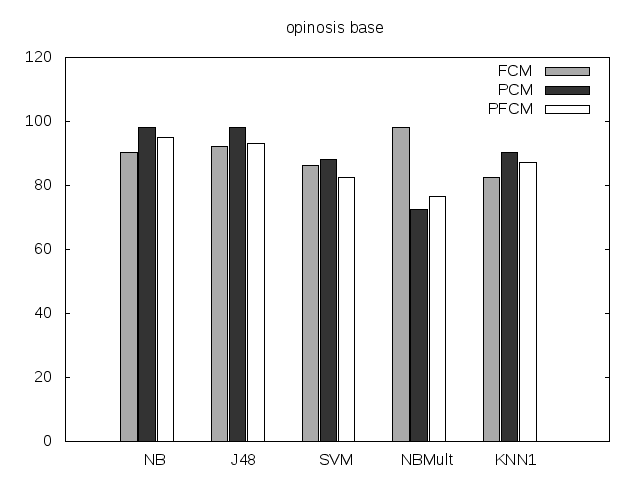
\includegraphics[width=1.0\columnwidth]{assets/pfcm/opinosis} 
    \caption{Desempenho obtido com os descritores extraídos com o algoritmo Soft-wFDCL a partir dos
      métodos de agrupamento FCM,
    PCM e PFCM executados na coleção Opinosis} 
  \label{fig:pfcmopinosis}
  \end{minipage}\hfill 
  \begin{minipage}{0.45\textwidth} \centering
    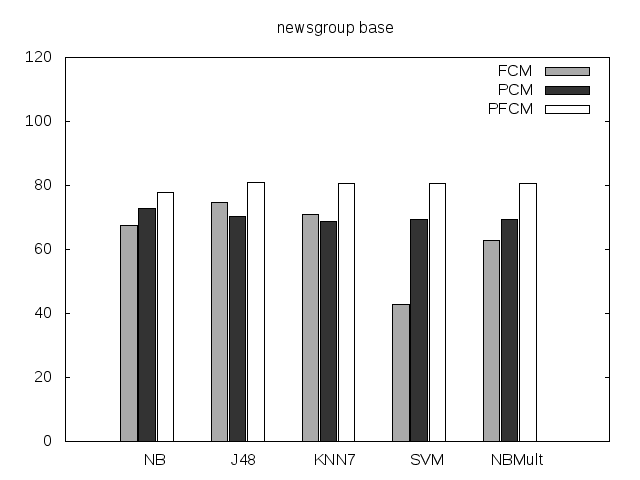
\includegraphics[width=1.0\columnwidth]{assets/pfcm/newsgroup} 
    \caption{Desempenho obtido com os descritores extraídos com o algoritmo Soft-wFDCL a partir dos
      métodos de agrupamento FCM,
    PCM e PFCM executados na coleção 20Newsgroup} 
     \label{fig:pfcm20news} 
   \end{minipage} 
\end{figure}

\begin{figure}[!htp] \centering 
   \begin{minipage}{0.45\textwidth} 
     \centering
    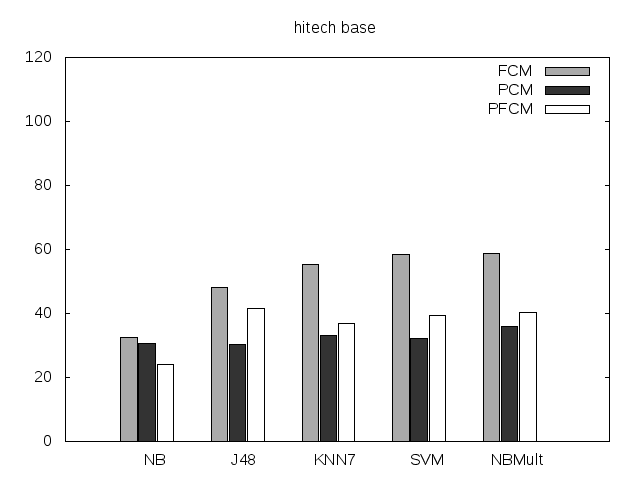
\includegraphics[width=1.0\columnwidth]{assets/pfcm/hitech} 
    \caption{Desempenho obtido com os descritores extraídos com o algoritmo Soft-wFDCL a partir dos
      métodos de agrupamento FCM,
    PCM e PFCM executados na coleção Hitech} 
  \label{fig:pfcmhitech}
  \end{minipage}\hfill 
  \begin{minipage}{0.45\textwidth} \centering
    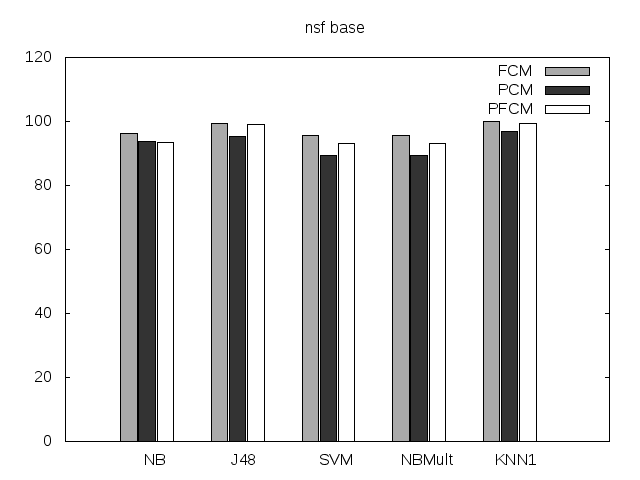
\includegraphics[width=1.0\columnwidth]{assets/pfcm/nsf} 
    \caption{Desempenho obtido com os descritores extraídos com o algoritmo Soft-wFDCL a partir dos
      métodos de agrupamento FCM,
    PCM e PFCM executados na coleção NSF} 
     \label{fig:pfcmnsf} 
   \end{minipage} 
\end{figure}

\begin{figure}[!htp] \centering 
   \begin{minipage}{0.45\textwidth} 
     \centering
    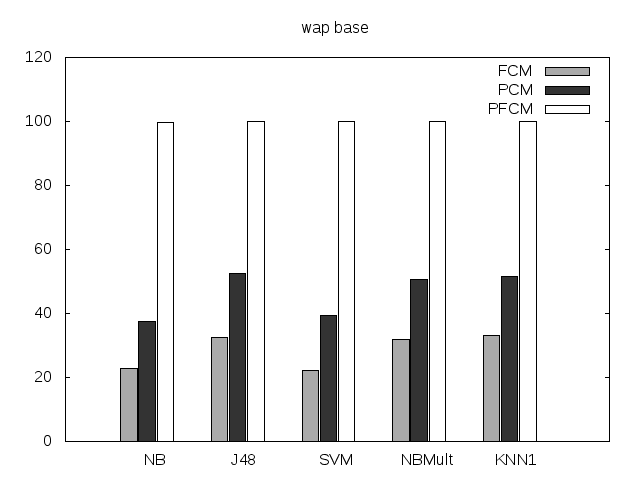
\includegraphics[width=1.0\columnwidth]{assets/pfcm/wap} 
    \caption{Desempenho obtido com os descritores extraídos com o algoritmo Soft-wFDCL a partir dos
      métodos de agrupamento FCM,
    PCM e PFCM executados na coleção WAP} 
    \label{fig:pfcmwap}
  \end{minipage}\hfill 
  \begin{minipage}{0.45\textwidth} \centering
    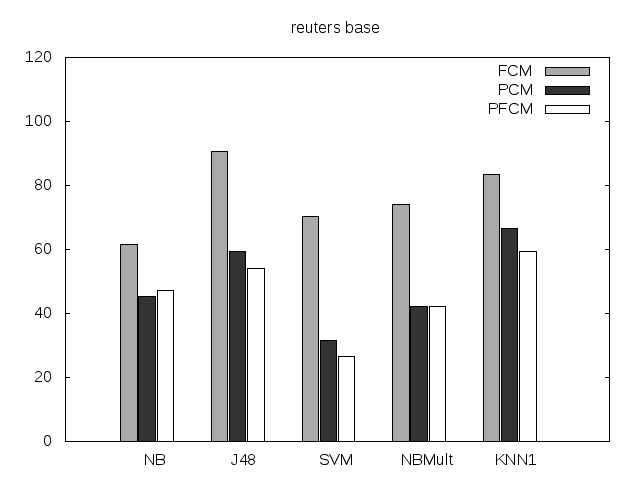
\includegraphics[width=1.0\columnwidth]{assets/pfcm/reuters} 
    \caption{Desempenho obtido com os descritores extraídos com o algoritmo Soft-wFDCL a partir dos
      métodos de agrupamento FCM,
    PCM e PFCM executados na coleção Reuters-21578} 
     \label{fig:pfcmreuters} 
   \end{minipage} 
\end{figure}

O resumo dos resultados do desempenho dos descritores extraídos após o agrupamento com os
algoritmos FCM, PCM e PFCM é apresentado na Tabela \ref{table:pfcmsummary}. Na tabela, a marcação
($\checkmark$) denota qual método de agrupamento obteve a maior taxa de classificação dentre os
demais.

\begin{table}[!htp]
  \centering
  \begin{tabular}{ |l|c c c c c c c c|}
    \hline
    {\bf nome} & docs & termos & classes & \% zeros & $>$ taxa & FCM & PCM & PFCM \\
    \hline
    {\bf Opinosis} & 51 & 842 & 3 & 95,73\% & 100,00\% & & $\checkmark$ &  \\
    \hline
    {\bf 20newsgroups} & 2000 & 11028 & 4 & 99,11\% & 81,20\% & & & $\checkmark$\\
    \hline
    {\bf Hitech} & 600 & 6925 & 6 & 97,93\% & 58,67\% & $\checkmark$ & & \\
    \hline
    {\bf NSF} & 1600 & 2806 & 16 & 99,76\% & 99,87\% & $\checkmark$ & & \\
    \hline
    {\bf WAP} & 1560 & 8070 & 20 & 98,51\% & 100\% & & & $\checkmark$ \\
    \hline
    {\bf Reuters-21578} & 1052 & 3925 & 43 & 98,55\% & 90,00\% & $\checkmark$ & & \\
    \hline
  \end{tabular}
  \caption{Sumário dos resultados da classificação dos descritores}
  \label{table:pfcmsummary}
\end{table}

Esses resultados obtidos reforçam a flexibilidade e adaptação do método Soft-wFDCL
\cite{Nogueira2013}, a novos algoritmos de agrupamento. De modo que o método se demonstra promissor
na tarefa extrair termos relevantes dos grupos produzidos na etapa de agrupamento, e isso é
demonstrado através do potencial preditivo evidenciado na Tabela \ref{table:pfcmsummary}, com as
taxas máximas de classificação de mais de 80\% para quase todas as bases, com exceção da base
Hitech, a qual obteve a taxa máxima de 58.67\%.  Por outro lado, ressalta-se a importância também de
avaliar de maneira subjetiva os descritores selecionados dos grupos, pois isso nos permite
compreender melhor se os termos obtidos fazem sentido. 

\begin{table}[!htp]
  \centering
  \begin{tabular}{ |l|p{4cm} | p{4cm} | p{4cm}|}
    \hline
    {\bf método} & $classe_1$ & $classe_2$ & $classe_3$ \\
    \hline
    {\bf FCM} & easy, clear, drive, display, control, car, version, nice, work, perfect & fact,
    import, isn't, model, problem, unit, design, don't, doesn't, found & breakfast, nearby,
    concierge, eat, bottle, coffee, floor, food, inn, friendly \\
    \hline
    {\bf PCM} & easy, read, problem, version, don't, small, nice, car, work, found & fact, back,
    turn, expect, size, close, quality, review, min, feature & feel, amazing, isn't, extreme, drive,
    include, point, reason, give, run\\
    \hline
    {\bf PFCM $\mu$} & easy, drive, control, don't, version, nice, car, work, perfect, lot & fact,
    isn't, read, complete, device, display, size, doesn't, found & breakfast, nearby, pleasant,
    concierge, eat, coffee, floor, clean, friendly, food\\
    \hline
    {\bf PFCM $\lambda$} & club, immaculate, send, towel, basic, exception, spotl, pillow, typical,
    fridge & pub, housekeep, holiday, tourist, tea, smoke, pm, renovate, facilite, london & usual,
    central, forum, bottle, modern, adult, supply, food, reserve, dinner\\
    \hline
  \end{tabular}
  \caption{Descritores extraídos com os métodos de agrupamento FCM, PCM e PFCM da coleção Opinosis,
  onde $\mu$ e $\lambda$ se referem as partições fuzzy e possibilística respectivamente, da qual os
descritores foram extraídos.}
  \label{table:pfcmdescriptors}
\end{table}

Para realizarmos uma análise subjetiva dos resultados, foi escolhido os descritores obtidos da base
de dados Opinosis, por possuir poucos grupos e assim facilitar a análise e a visualização. A coleção
Opinosis contém opiniões dos usuários a respeito de serviços de hospedagem, dispositivos eletrônicos
e carros.  Portanto na Tabela \ref{table:pfcmdescriptors} temos a seleção de termos descritores
escolhidos para cada grupo, pelos respectivos métodos de agrupamento. Ao analisarmos os termos
selecionados é possível notar uma tendência geral, da $classe_1$ conter palavras relacionadas a
carros, a $classe_2$ abordando opiniões dos usuários sobre dispositivos eletrônicos e a $classe_3$
com opiniões a respeito dos serviços de hospedagem e alimentação. Contudo nota-se que os descritores
do PCM e do PFCM$\lambda$ (descritores da partição possibilística do PFCM) estão um pouco mais
misturados, não apresentando uma tendência geral bem definida. Uma explicação possível a esse
resultado, pode se encontrar na própria partição possibilística a qual permite que um mesmo
documento possua um grau de tipicidade elevado em todos os grupos. Portanto uma solução possível,
pode ser uma adaptação do método de extração de descritores Soft-wFDCL voltado para a partição
possibilística, assim como também para algoritmos híbridos com duas partições, que é o caso do PFCM.

De maneira complementar, é importante salientar que o método de extração de descritores Soft-wFDCL é
totalmente influenciado pelos valores contidos nas partições fuzzy e possibilística. Portanto, é
também importante se realizar uma análise dos métodos de agrupamento utilizados no experimento, com
a finalidade de se entender qual método é mais apropriado em determinados contextos. Nesse contexto
os resultados apontam que a dimensionalidade das bases foi um fator determinante no desempenho dos
métodos de agrupamento no contexto da organização flexível de documentos, e consequentemente a
extração de descritores. Por exemplo, do sumário de resultados apresentados na Tabela
\ref{table:pfcmsummary}, podemos observar que a o método PCM obteve o melhor resultado na coleção
Opinosis, que possui a menor dimensionalidade (842 termos), enquanto que o algoritmo FCM superou os
demais métodos nas bases NSF (2806 termos), Reuters-21578 (3925 termos), Hitech (6925 termos), e por
fim o algoritmo PFCM atingiu melhores resultados para as bases WAP (8070 termos) e 20Newsgroup
(11028 termos), que são as bases de maior dimensionalidade na coleção.

Na próxima sessão, motivado pelos resultados desse experimento será explorado uma adaptação do
método Soft-wFDCL para evitar o processo de extração dupla de descritores em algoritmos que possuam
partições fuzzy e possibilística.

\section{Método Mixed-PDCL}

Uma das conclusões do experimento anterior, foi acerca do problema ao se realizar a extração dos
descritores individualmente em cada partição do PFCM, que por sua vez é utiliza uma abordagem mista.
Logo, é intuitivo indagar, que para uma melhor interpretação dos grupos produzidos em um método de
agrupamento híbrido, seja pertinente utilizar também uma abordagem mista de extração descritores.
Aproveitando-se assim dos benefícios existentes na partição possibilística, a qual penaliza os
elementos ruidosos, com baixos valores de tipicidade, sem abrir mão das vantagens presentes na
partição fuzzy. Para isso é necessário se compreender os mecanismos de funcionamento do método
Soft-wFDCL, para que seja possível propor uma adaptação para este cenário.

\section{Método HPCM}
\section{Considerações finais}


\xchapter{Conclusão}{Síntese da investigação e dos experimentos realizados nesta monografia}

A pesquisa desenvolvida nesta monografia investiga e elabora uma solução voltada para organização
de uma coleção de documentos textuais de maneira flexível. O processo de organização em si, conforme 
discutido ao longo dos capítulos, envolve uma gama de desafios para ser executado com eficiência, como, 
por exemplo, os impactos negativos da elevada dimensionalidade da matriz documentos x termos, que 
é comumente muito esparsa em coleções textuais. Por conta disso, a tarefa de se calcular a similaridade
entre dois documentos quaisquer, a partir daquela mesma matriz, apresenta alto grau de dificuldade. 
Outro problemática fundamental está no processo de agrupamento, através do qual se espera que os grupos resultantes 
consigam capturar a estrutura natural das coleções e que esses grupos possuam relevância para os usuários finais. 
Atendendo a esses princípios, o agrupamento consegue cumprir o papel de aquisição e descoberta de conhecimento. Coleções textuais podem também 
conter documentos ruidosos, que destoam do restante da coleção, sendo que é esperado o emprego de técnicas no processo de organização
flexível para que ele não seja prejudicado pela presença desses documentos. Com o aumento massivo da
quantidade de dados produzidos pela humanidade, se faz também necessário que todo o processo seja
capaz de se adequar a coleções com grande volumes de dados. Assim, a organização flexível de documentos proposta fundamenta-se em um conhecimento 
bastante intensivo, por meio do qual se aplica um conjunto de diversas técnicas os desafios apontados acima bem como outros associados a 
esse processamento de textos. Parte relevante das técnicas aqui empregadas derivam dos estudos demineração de textos e, consequentemente, 
também da mineração de dados. 

Todo esse contexto apresentado se mostra inviável de ser abordado de maneira aprofundada em uma única
pesquisa. Por isso, as investigações conduzidas nessa monografia foram focadas no aumento da
robustez do processo, reduzindo-se os impactos dos dados ruidosos ao se utilizar uma estratégia
híbrida com o algoritmo PFCM. Portanto, a hipótese formulada e verificada nesta monografia foi:

\begin{quote}
\textit{A utilização de uma estratégia híbrida de agrupamento e extração de descritores, entre os 
  graus de pertinência e tipicidade providos pelo método de agrupamento PFCM, permitem o aumento da
    robustez e resiliência contra ruídos na organização flexível de documentos, aumentando assim a
    relevância dos grupos obtidos.}
\end{quote}

Portanto, com base na exploração das estratégias existentes na literatura para aprimoramento do
processo de organização flexível de documentos e da avaliação da hipótese formulada, o objetivo
desta monografia é definido como segue:

\begin{quote}
\textit{Conduzir uma investigação em torno dos métodos de agrupamento FCM, PCM e PFCM, para
se compreender e interpretar corretamente as peculiaridades de se extrair descritores em um
agrupamento híbrido.}
\end{quote}

A fim de atender a esse objetivo, foi realizado nesta monografia um estudo dos fundamentos
necessários para a organização flexível de documentos, uma revisão das estratégias recentes
utilizadas por pesquisadores para aprimorar a organização flexível de documentos. E, por fim, como
resultado, o estudo dos impactos de se utilizar o algoritmo PFCM no processo e na extração de
descritores, o qual derivaram a proposição de dois métodos de extração de descritores: PDCL e
Mixed-PFDCL. Tais métodos são extensões do método SoftO-FDCL apresentado em \cite{Nogueira2013}, e
diante dos resultados, contribuem de maneira significativa para o estado da arte da extração de
descritores dos grupos fuzzy.

Na seção seguinte, apresentam-se as principais contribuições fornecidas por esta monografia e os
possíveis trabalhos futuros que derivam desta pesquisa.

\section{Resumo das contribuições}

A investigação realizada nesta monografia, produziu algumas importantes contribuições para o
processo de se organizar documentos de maneira flexível. Essas contribuições são distribuídas no estudo e
fundamentação da teoria relacionada a esse campo de estudo, investigação e apresentação das
possibilidades de aprimoramento e otimização do processo explorados recentemente na literatura e a
investigação das peculiaridades de adotar uma estratégia híbrida o que posteriormente motivou a
proposição de dois métodos de extração de descritores. 

A partir do estudo da teoria e dos fundamentos necessários para o tema, é apresentado nesta
monografia um rico conteúdo abordando os detalhes dos métodos de agrupamento FCM, PCM, PFCM e HFCM,
juntamente com os seus pseudo-códigos, para auxiliar novos pesquisadores na rápida implementação de
tais métodos.

Outra importante contribuição, consiste na apresentação das pesquisas que se situam no estado da
arte das etapas presentes no processo de organização flexível de documentos. Ficou evidenciado, a
partir das pesquisas encontradas na literatura, a diversidade as estratégias existentes na literatura
para mitigar os desafios existentes. Foi visto que ainda é proposto abordagens para aprimorar todas
as etapas existentes no processo, as quaiscontemplam o pré-processamento, agrupamento, extração
de descritores e recuperação da informação, com isso conclui-se que a organização flexível não é um
problema resolvido na literatura, o que o torna um problema de pesquisa bastante promissor. 

A primeira contribuição experimental dessa monografia, consistiu no estudo dos impactos de se
adicionar o método PFCM no processo de organização flexível de documentos. A partir desse estudo
foi observado que o algoritmo PFCM possui uma tendência para aumentar a eficiência do
agrupamento produzido em coleções textuais de maior dimensionalidade, o que foi comprovado a partir
das evidências contidas na Tabela \ref{table:pfcmsummary}. No entanto, se destaca aqui a importância
da realização de novos estudos com um maior número de coleções textuais de baixa e alta
dimensionalidade para se confirmar esta tendência. 

Por outro lado, constatou-se nesse experimento a capacidade de adaptação do método
SoftO-FDCL a novos algoritmos de agrupamento. No entanto, este último método, segundo as suas pesquisas iniciais, considera somente uma única
partição no processo de pontuação dos termos candidatos, o que por sua vez não consegue capturar
toda a essência do agrupamento produzido pelo PFCM. Ainda nesse experimento foi observado um
problema na interpretação das tipicidades contidas em partições possibilísticas, no processo de
extração de descritores. Esse problema deriva diretamente da natureza probabilística dos graus de
pertinência da partição fuzzy do FCM, que não se aplica às tipicidades, a qual influencia
direta adequação ou não do limiar $\delta$ do método SoftO-FDCL. 

Portanto, a partir da identificação desse problema de interpretação dos graus de compatibilidade
possibilísticos, uma outra importante contribuição dessa monografia, consiste na formulação das
propriedades do limiar apresentadas nas equações \ref{eq:limiarp1}, \ref{eq:limiarp2} e
\ref{eq:limiarp3}. Essas propriedades expressam características importantes, que os graus de
compatibilidade devem possuir, para o limiar $\delta$ do método do método SoftO-FDCL conseguir
extrair bons descritores dos grupos. 

Feitas essas considerações, apresentam-se as duas principais contribuições dessa monografia. A primeira consiste no
método PDCL, que propõe uma abordagem para interpretar os graus de compatibilidade possibilísticos,
respeitando as propriedades das equações \ref{eq:limiarp1}, \ref{eq:limiarp2} e \ref{eq:limiarp3},
sem deixar de lado a resiliência contra ruídos inerente das tipicidades. Os experimentos conduzidos
com esse método demonstraram a qualidade dos descritores extraídos com o PDCL em comparação com o
método SoftO-FDCL, cujos comparativos estão apresentados na Tabela \ref{table:rankingpdcl}. No entanto, observou-se
neste experimento que o método PCM produziu uma quantidade baixa de grupos em comparação ao número
total de classes em cada coleção, assim como também a defuzificação resultou em grupos majoritários
com elevado percentual. Com isso, é importante salientar, a necessidade de se conduzir estudos
experimentais a respeito dos parâmetros ideais dos métodos de agrupamento para coleções textuais.

A segunda grande contribuição desta monografia consiste na proposta de um método de extração de
descritores híbrido, capaz de interpretar as duas partições presentes no algoritmo PFCM de maneira
bastante satisfatória. Um segundo experimento foi então conduzido para atestar os
benefícios desse abordagem híbrida de extração de descritores. Os resultados apresentados no sumário
da Tabela \ref{table:pdclsummary}, atestam através de uma avaliação preditiva com clássicos
algoritmos de classificação, que os descritores extraídos através do método Mixed-PFDCL no
agrupamento resultante do método PFCM, foram melhores que os descritores do método SoftO-FDCL.
Ainda na Tabela \ref{table:rankingmixedpdcl}, se demonstrou que os descritores obtidos com o método
Mixed-PFDCL preservam uma proximidade semântica, com os demais termos do mesmo grupo, assim como os
descritores do método SoftO-FDCL.

Durante as pesquisas realizadas neste projeto de conclusão de curso, houve a publicação de um artigo
com os resultados obtidos no primeiro experimento, em uma das mais importantes conferências de
sistemas fuzzy. Isso reforça a importância e relevância do tema estudado nesta monografia para a
comunidade científica. Segue o artigo publicado:
\begin{quote}
CARVALHO, N. V. J. et al. Flexible Document Organization by Mixing Fuzzy and Possibilistic
Clustering algorithms. IEEE International Conference on Fuzzy Systems (FUZZ- IEEE), p. 1–8, 2016.
\end{quote}

\section{Trabalhos futuros}

Ao considerar todas as conclusões apresentadas anteriormente, existem diversas possibilidades que
podem derivar deste trabalho. Em particular, foi notado que é necessário se realizar uma avaliação
mais apurada dos impactos na variação dos parâmetros dos algoritmos de agrupamento, de modo que se
possa obter, senão uma forma automatizada dos parâmetros com base nas características das bases,
pelo menos indicações de quais parâmetros utilizar. 

Nesse sentido, está apresentado na Figura \ref{fig:pfcmvarying}, um exemplo dos impactos da variação
da quantidade de grupos e do parâmetro $m$, sobre a medida de silhueta fuzzy. Ao analisar o gráfico,
observa-se uma clara tendência da medida de silhueta fuzzy (FS) aumentar, com o incremento no número
de grupos e para a faixa de valores de $m$ entre 1,0 e 1,4. Contudo, esse tipo de análise requer
sucessivas execuções de todo o agrupamento, o que por sua vez é um processo bastante oneroso
computacionalmente. Sendo assim, pretende-se estender esse estudo para outras bases e para os
demais algoritmos de agrupamento, assim como mensurar a qualidade do agrupamento produzido
através de outras medidas de validação existentes na literatura, como, por exemplo, as medidas de
entropia e pureza do agrupamento apresentadas em \citeonline{Deepa2012} ou a medida de validação
proposta em \citeonline{ZhangZhou2008}, que explora as pertinências e tipiciadades existentes no
PFCM.

\begin{figure}[!h] \centering 
  \centering
  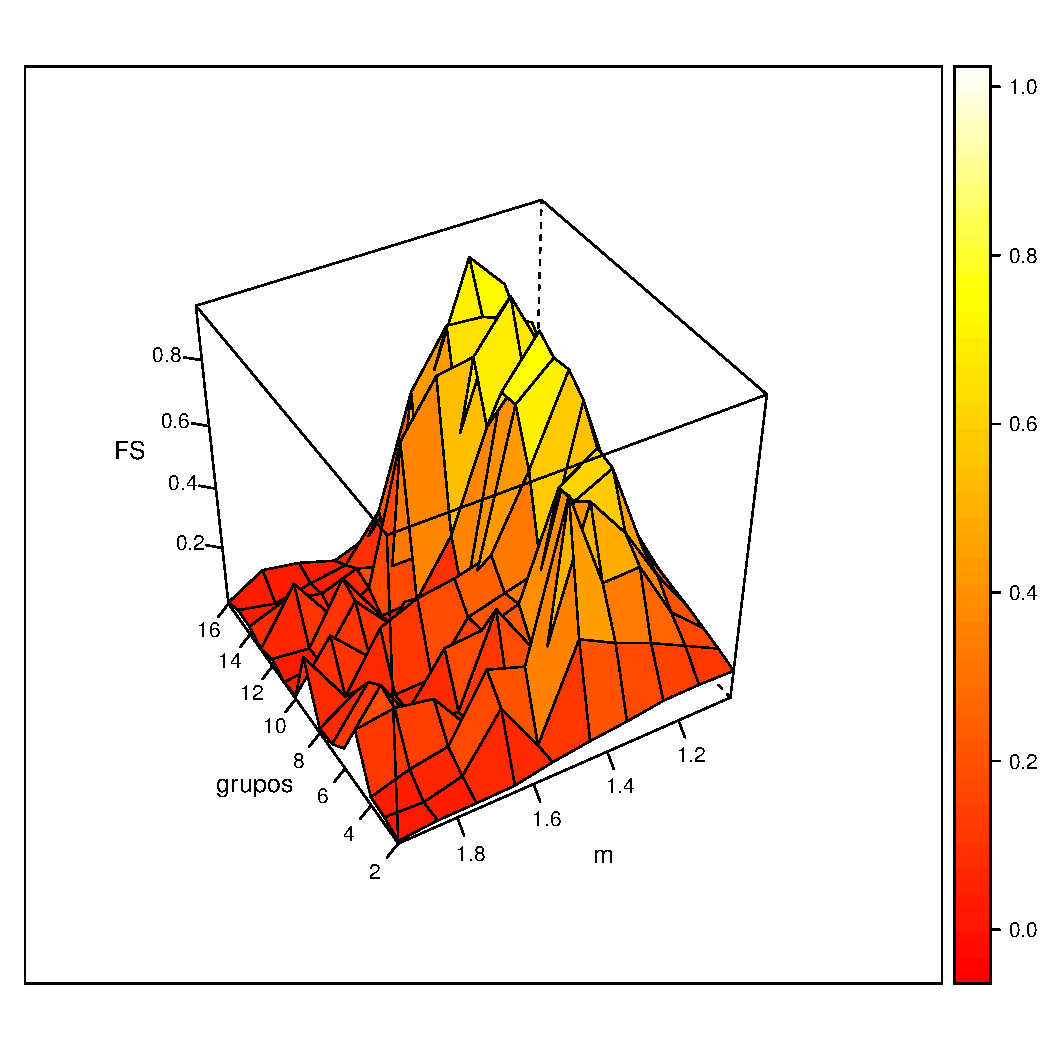
\includegraphics[width=0.8\columnwidth]{assets/future_works/pfcm_nsf_varying.pdf} 
  \caption{Gráfico das influências da variação da quantidade de grupos e do parâmetro $m$, na
pontuação obtida pela medida de silhueta fuzzy para o algoritmo PFCM na base NSF} 
  \label{fig:pfcmvarying}
\end{figure}

Nesta monografia, também foi observado diversas vezes que um dos grandes desafios no agrupamento de
documentos está na dimensionalidade dos dados. Soma-se a isso o fato de que os principais algoritmos
de agrupamento possuem como ponto crítico de decisão no processo de separação dos elementos em
grupos, a medida de similaridade. Sendo assim, é importante se investigar também as possibilidades de
aprimoramento da organização flexível de documentos com as recentes medidas de similaridade
propostas na literatura \cite{Lin2014,Nagwani2015} para dados de alta dimensionalidade e em
particular para coleções textuais.

Outro aspecto de grande relevância é a escalabilidade da proposta de organização flexível de
documentos, para coleções textuais que se enquadram na categoria {\it Very Large\/} de acordo com a
Tabela \ref{table:datasize}. Portanto, se pretende realizar estudos objetivando escalar o processo
utilizado nesta pesquisa para o cenário de {\it Big Data\/}, utilizando como base as pesquisas com
grandes quantidades de dados apresentadas em \citeonline{Honda:2014}, \citeonline{Wang:2014} e
\citeonline{Havens2012}. De antemão, postula-se que, no que diz respeito a implementação dos algoritmos
aqui utilizados, todo o processo deve ter sido paralelizado utilizando o framework de computação paralela
OpenMP ({\it Open Multi-Processing\/})\footnotemark, o que habilita a realização de experimentos em
computadores com elevado potencial de processamento.
\footnotetext{\url{http://openmp.org/}}



\xchapter{Trabalhos Futuros}{Possíveis explorações adicionais que derivam deste trabalho}

% DESCRIBE EXPLORATIONS TO THIS RESEARCH


%% Parte pos-textual
\backmatter

% Apendices
% Comente se naoo houver apendices
\appendix

% Eh aconselhavel criar cada apendice em um arquivo separado, digamos
% "apendice1.tex", "apendice.tex", ... "apendiceM.tex" e depois
% inclui--los com:
% \include{apendice1}
% \include{apendice2}
% ...
% \include{apendiceM}

% Bibliografia
% É aconselhável utilizar o BibTeX a partir de um arquivo, digamos "biblio.bib".
% Para ajuda na criação do arquivo .bib e utilização do BibTeX, recorra ao
% BibTeXpress em www.cin.ufpe.br/~paguso/bibtexpress
\bibliographystyle{abntex2-alf}
\bibliography{biblio}

%% Fim do documento
\end{document}
%------------------------------------------------------------------------------------------%
